\documentclass{standalone}
\usepackage{tikz}
\usetikzlibrary{patterns, positioning}


\begin{document}
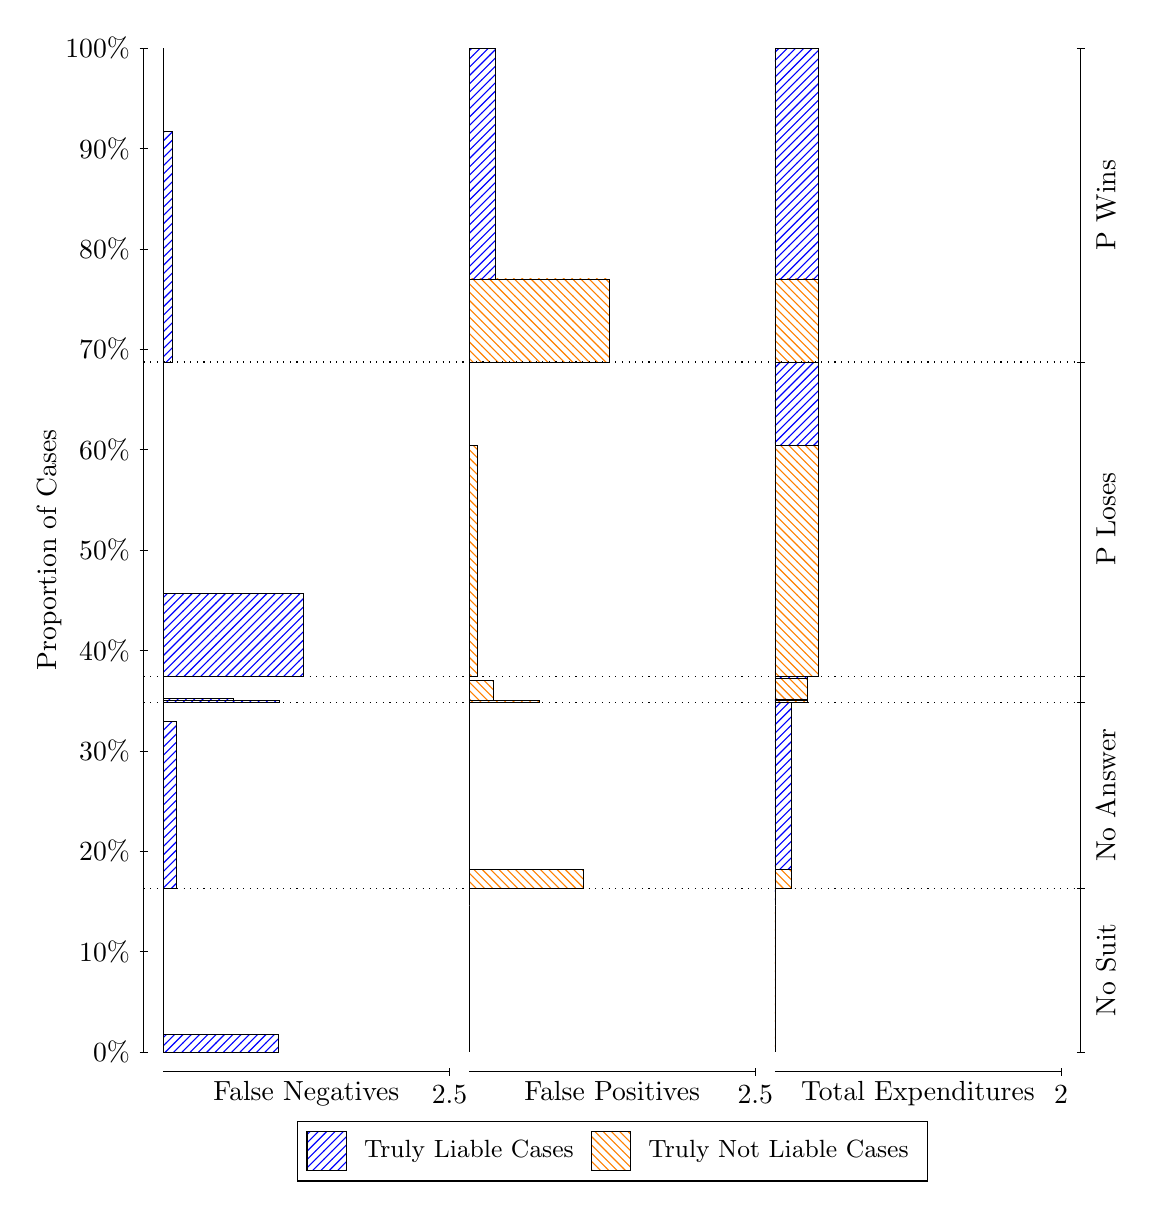
\begin{tikzpicture}
\draw[black, very thin] (1.5,1.75) -- (1.5,14.5);
\node[rotate=90, text=black, anchor=center] at (0.3, 8.125) {Proportion of Cases};
\draw[black, very thin] (1.45,1.75) -- (1.55,1.75);
\node[text=black, anchor=east] at (1.45, 1.75) {0\%};
\draw[black, very thin] (1.45,3.025) -- (1.55,3.025);
\node[text=black, anchor=east] at (1.45, 3.025) {10\%};
\draw[black, very thin] (1.45,4.3) -- (1.55,4.3);
\node[text=black, anchor=east] at (1.45, 4.3) {20\%};
\draw[black, very thin] (1.45,5.575) -- (1.55,5.575);
\node[text=black, anchor=east] at (1.45, 5.575) {30\%};
\draw[black, very thin] (1.45,6.85) -- (1.55,6.85);
\node[text=black, anchor=east] at (1.45, 6.85) {40\%};
\draw[black, very thin] (1.45,8.125) -- (1.55,8.125);
\node[text=black, anchor=east] at (1.45, 8.125) {50\%};
\draw[black, very thin] (1.45,9.4) -- (1.55,9.4);
\node[text=black, anchor=east] at (1.45, 9.4) {60\%};
\draw[black, very thin] (1.45,10.675) -- (1.55,10.675);
\node[text=black, anchor=east] at (1.45, 10.675) {70\%};
\draw[black, very thin] (1.45,11.95) -- (1.55,11.95);
\node[text=black, anchor=east] at (1.45, 11.95) {80\%};
\draw[black, very thin] (1.45,13.225) -- (1.55,13.225);
\node[text=black, anchor=east] at (1.45, 13.225) {90\%};
\draw[black, very thin] (1.45,14.5) -- (1.55,14.5);
\node[text=black, anchor=east] at (1.45, 14.5) {100\%};

\draw[black, very thin] (13.4,1.75) -- (13.4,14.5);
\draw[black, very thin] (13.35,1.75) -- (13.45,1.75);
\node[anchor=west] at (13.35, 1.75) {};
\draw[black, very thin] (13.35,3.8317) -- (13.45,3.8317);
\node[anchor=west] at (13.35, 3.8317) {};
\draw[black, very thin] (13.35,6.1889) -- (13.45,6.1889);
\node[anchor=west] at (13.35, 6.1889) {};
\draw[black, very thin] (13.35,6.524) -- (13.45,6.524);
\node[anchor=west] at (13.35, 6.524) {};
\draw[black, very thin] (13.35,10.512) -- (13.45,10.512);
\node[anchor=west] at (13.35, 10.512) {};
\draw[black, very thin] (13.35,14.5) -- (13.45,14.5);
\node[anchor=west] at (13.35, 14.5) {};

\draw[black, very thin, pattern color=blue, pattern=north east lines] (1.75,1.75) rectangle (3.2033,1.969);
\draw[black, very thin, pattern color=orange, pattern=north west lines] (1.75,1.969) rectangle (1.75,3.8317);
\draw[black, very thin, pattern color=blue, pattern=north east lines] (1.75,3.8317) rectangle (1.9135,5.9468);
\draw[black, very thin, pattern color=orange, pattern=north west lines] (1.75,5.9468) rectangle (1.75,6.1889);
\draw[black, very thin, pattern color=blue, pattern=north east lines] (1.75,6.1889) rectangle (3.2215,6.2157);
\draw[black, very thin, pattern color=blue, pattern=north east lines] (1.75,6.2157) rectangle (2.9308,6.2184);
\draw[black, very thin, pattern color=blue, pattern=north east lines] (1.75,6.2184) rectangle (2.6402,6.2417);
\draw[black, very thin, pattern color=orange, pattern=north west lines] (1.75,6.2417) rectangle (1.75,6.524);
\draw[black, very thin, pattern color=blue, pattern=north east lines] (1.75,6.524) rectangle (3.5303,7.5787);
\draw[black, very thin, pattern color=orange, pattern=north west lines] (1.75,7.5787) rectangle (1.75,10.512);
\draw[black, very thin, pattern color=blue, pattern=north east lines] (1.75,10.512) rectangle (1.859,13.445);
\draw[black, very thin, pattern color=orange, pattern=north west lines] (1.75,13.445) rectangle (1.75,14.5);
\draw[black, very thin, pattern color=orange, pattern=north west lines] (5.6333,1.75) rectangle (5.6333,3.6127);
\draw[black, very thin, pattern color=blue, pattern=north east lines] (5.6333,3.6127) rectangle (5.6333,3.8317);
\draw[black, very thin, pattern color=orange, pattern=north west lines] (5.6333,3.8317) rectangle (7.0867,4.0737);
\draw[black, very thin, pattern color=blue, pattern=north east lines] (5.6333,4.0737) rectangle (5.6333,6.1889);
\draw[black, very thin, pattern color=orange, pattern=north west lines] (5.6333,6.1889) rectangle (6.5235,6.2121);
\draw[black, very thin, pattern color=orange, pattern=north west lines] (5.6333,6.2121) rectangle (6.2328,6.2181);
\draw[black, very thin, pattern color=orange, pattern=north west lines] (5.6333,6.2181) rectangle (5.9422,6.4712);
\draw[black, very thin, pattern color=blue, pattern=north east lines] (5.6333,6.4712) rectangle (5.6333,6.524);
\draw[black, very thin, pattern color=orange, pattern=north west lines] (5.6333,6.524) rectangle (5.7423,9.4574);
\draw[black, very thin, pattern color=blue, pattern=north east lines] (5.6333,9.4574) rectangle (5.6333,10.512);
\draw[black, very thin, pattern color=orange, pattern=north west lines] (5.6333,10.512) rectangle (7.4137,11.567);
\draw[black, very thin, pattern color=blue, pattern=north east lines] (5.6333,11.567) rectangle (5.9603,14.5);
\draw[black, very thin, pattern color=orange, pattern=north west lines] (9.5167,1.75) rectangle (9.5167,3.6127);
\draw[black, very thin, pattern color=blue, pattern=north east lines] (9.5167,3.6127) rectangle (9.5167,3.8317);
\draw[black, very thin, pattern color=orange, pattern=north west lines] (9.5167,3.8317) rectangle (9.721,4.0737);
\draw[black, very thin, pattern color=blue, pattern=north east lines] (9.5167,4.0737) rectangle (9.721,6.1889);
\draw[black, very thin, pattern color=orange, pattern=north west lines] (9.5167,6.1889) rectangle (9.9254,6.2121);
\draw[black, very thin, pattern color=blue, pattern=north east lines] (9.5167,6.2121) rectangle (9.9254,6.2354);
\draw[black, very thin, pattern color=orange, pattern=north west lines] (9.5167,6.2354) rectangle (9.9254,6.4945);
\draw[black, very thin, pattern color=blue, pattern=north east lines] (9.5167,6.4945) rectangle (9.9254,6.524);
\draw[black, very thin, pattern color=orange, pattern=north west lines] (9.5167,6.524) rectangle (10.062,9.4574);
\draw[black, very thin, pattern color=blue, pattern=north east lines] (9.5167,9.4574) rectangle (10.062,10.512);
\draw[black, very thin, pattern color=orange, pattern=north west lines] (9.5167,10.512) rectangle (10.062,11.567);
\draw[black, very thin, pattern color=blue, pattern=north east lines] (9.5167,11.567) rectangle (10.062,14.5);
\draw[black, dotted] (1.5,3.8317) -- (13.4,3.8317);
\draw[black, dotted] (1.5,6.1889) -- (13.4,6.1889);
\draw[black, dotted] (1.5,6.524) -- (13.4,6.524);
\draw[black, dotted] (1.5,10.512) -- (13.4,10.512);
\draw[black, very thin] (1.75,1.5) -- (5.3833,1.5);
\node[text=black, anchor=north] at (3.5667, 1.5) {False Negatives};
\draw[black, very thin] (5.3833,1.45) -- (5.3833,1.55);
\node[text=black, anchor=north] at (5.3833, 1.45) {2.5};

\draw[black, very thin] (5.6333,1.5) -- (9.2667,1.5);
\node[text=black, anchor=north] at (7.45, 1.5) {False Positives};
\draw[black, very thin] (9.2667,1.45) -- (9.2667,1.55);
\node[text=black, anchor=north] at (9.2667, 1.45) {2.5};

\draw[black, very thin] (9.5167,1.5) -- (13.15,1.5);
\node[text=black, anchor=north] at (11.333, 1.5) {Total Expenditures};
\draw[black, very thin] (13.15,1.45) -- (13.15,1.55);
\node[text=black, anchor=north] at (13.15, 1.45) {2};

\node[text=black, centered, rotate=90] at (13.72, 2.7908) {No Suit};
\node[text=black, centered, rotate=90] at (13.72, 5.0103) {No Answer};

\node[text=black, centered, rotate=90] at (13.72, 8.518) {P Loses};
\node[text=black, centered, rotate=90] at (13.72, 12.506) {P Wins};

\draw (7.449999999999999,1.5) node[draw=none] (baseCoordinate) {};
\begin{scope}[align=center]
        \matrix[scale=0.5, draw=black, below=0.5cm of baseCoordinate, nodes={draw}, column sep=0.1cm]{
            \node[rectangle, draw, minimum width=0.5cm, minimum height=0.5cm, pattern color=blue, pattern=north east lines] {}; &
            \node[draw=none, font=\small, text=black] (B) {Truly Liable Cases}; &
            \node[rectangle, draw, minimum width=0.5cm, minimum height=0.5cm, pattern color=orange, pattern=north west lines] {}; &
            \node[draw=none, font=\small, text=black] (B) {Truly Not Liable Cases}; \\
            };
\end{scope}

\end{tikzpicture}
\end{document}